%% tags: poster, anchor, doubleBoundary, double accept, variables
\PassOptionsToPackage{usenames,dvipsnames}{xcolor}
\documentclass[tikz,border=2]{standalone}
% FONTS
\usepackage{gillius2}
\renewcommand{\familydefault}{\sfdefault}
%% \renewcommand*\familydefault{\sfdefault}
%% \usepackage[scaled]{helvet}
\usepackage{microtype} % some compression
%% \usepackage{bold-extra} % for bold and textsc
% MATH
\usepackage{amssymb}
\usepackage{mathtools} % contains amsmath which comes with align
\usepackage{amsthm}
\usepackage{enumitem}
\usepackage{graphicx}
\usepackage[skins]{tcolorbox}
\setlist[itemize]{label=\textcolor{gray}{\tiny{$\blacksquare$}},leftmargin=*,itemsep=.05em,topsep=0pt}
%%%%%%%%%%
\definecolor{hokie}{RGB}{142,35,68}
\definecolor{blue1}{HTML}{93A7B3}
\definecolor{blue2}{HTML}{557082}
\definecolor{blue3}{HTML}{3C5B6F}
\definecolor{cream1}{HTML}{F5F5EB}
\definecolor{cream2}{HTML}{EDEADA}
\definecolor{gray1}{HTML}{C2C1BA}
%%
\newcommand{\tuta}{\emph{T. absoluta}}
\newcommand{\secLine}[2]{\draw[line width=.15cm, draw=blue1] ($(#1.south
west)+(0,0)$) -- +(#2,0);}
%%
\usetikzlibrary{shadows,arrows,shapes,positioning,calc,backgrounds,
fit,automata,decorations.markings,
decorations.pathreplacing,decorations.pathmorphing,spy}
%%%%%%%%%%%%%%%%%%%%%%%
\begin{document}
\begin{tikzpicture}
   [scale=2.54,auto,x=1cm,y=1cm, 
   block/.style={rectangle,draw=black,minimum width=10cm,minimum height=8cm},
   arr/.style={>=latex', shorten >=.0pt, shorten <=.0pt},
   every node/.style={align=left},
   accept/.style={double,double distance=4pt,circle,draw=blue2,fill=blue2},
   acceptSmall/.style={accept,inner sep=2pt},
   fig/.style={draw=blue2,fill=white,thick,inner sep=2pt},
   section/.style={font=\LARGE,color=black},
   subsection/.style={section,font=\Large,color=blue2},
   body/.style={anchor=north west,font=\normalsize,text width=10.5cm},
   transform shape, spy using outlines={rectangle,connect
   spies,draw=gray,ultra thick,magnification=2}]
\def\secSep{-.3}
% main rectangle to fix shape
\node[block,draw=black,minimum width=35cm,minimum height=30cm] (main) {};
% anchor points
\node[anchor=north west] (topLeft) at ($(main.north west)+(.2,-.2)$) {};
\node[anchor=south east] (botRight) at ($(main.south east)+(-.2,.2)$) {};
% title block
%%
\node[anchor=north west,section,color=blue2,font=\Huge\bfseries,text
width=22cm] (title) at (topLeft.north west)
{Towards an Integrated Network-based Approach to \\\vspace{-.1cm}
Modeling the Dynamics of Invasive Plant Pests};
%%
\node[section,anchor=north west,font=\Large,blue2,shift={(0,0)}] at (title.south west) (authors) 
{S.~Venkatramanan,$^\dagger$ \textbf{A.~Adiga},$^\dagger$
A.~Marathe,$^\dagger$ S.~Eubank,$^\dagger$ M.~Marathe,$^\dagger$ and
R.~Muniappan$^*$};
%%
\node[body,font=\Large,text width=21cm,shift={(0,0)}] (inst) at
(authors.south west)
{$^\dagger$Network Dynamics and Simulation Science Laboratory, Biocomplexity
Institute of Virginia Tech \\
$^*$IPM Innovation Lab, Virginia Tech};
%%
\node[anchor=north east,shift={(0,-.5)}] (bivt) at (topLeft.north-|botRight.east)
{\includegraphics[height=1.25cm]{aux/bivt_logo.pdf}};
\node[anchor=north east,shift={(-.5,-.1)}] (ndssl) at (bivt.north west)
{\includegraphics[height=1cm]{aux/ndssl_logo.png}};
\node[below=of ndssl,shift={(0,1)}] (ftf)
{
\includegraphics[height=1.6cm]{aux/ftf.pdf}};
\node[below=of bivt,shift={(0,1)}] (usaid)
{\includegraphics[height=1.3cm]{aux/usaid.pdf}};
\node[left of=ndssl,shift={(-3.5,-.8)}] (ipmil) {\includegraphics[width=2.7cm]{aux/ipm-il.pdf}};
\def\yspace{-4.8cm}
\def\xspace{7cm}
%% intro1
\node[section,anchor=north west,shift={(0,-.2)}] (background) at
(inst.south west) {Background};
\secLine{background}{7cm}
\node[body,anchor=north west] (backgroundBody) at (background.south west) {
Globally, invasive alien species pose a growing threat to native
ecosystems, health, food security and economic stability.};
%%
\node[section,anchor=north west,shift={(0,\secSep)}] (problem) at
(backgroundBody.south west) {Problem};
\secLine{problem}{7cm}
%%
\node[body,anchor=north west] (problemBody) at (problem.south west) {
The dynamics of biological invasions, particularly pests and pathogens
associated with agricultural crops, are influenced not only by biological
and climatic factors, but also human-centric activities such as trade,
travel, supply chains, agricultural practices, etc. How do we model such a
complex phenomenon?
};
%%
\node[section,anchor=north west,shift={(0,\secSep)}] (challenge) at (problemBody.south west) {Challenges};
\secLine{challenge}{7cm}
\node[body] (challengeBody) at (challenge.south west) {
Modeling invasive species dynamics requires 
\begin{itemize}
   \item expertise from various disciplines
   \item integrating data of different types and from multiple sources;
   incomplete and noisy
   \item integrating models that represent all possible pathways of spread
   \item more complex the model, the harder it is to calibrate, verify and
   validate
\end{itemize}
};
%%
\node[section,anchor=north west,shift={(0,\secSep)}] (approach) at
(challengeBody.south west) {Our approach};
\secLine{approach}{7cm}
%%
\node[body,anchor=north west] (approachBody) at (approach.south west) {
We envision a modeling paradigm for building realistic models of spread
\begin{itemize}
\item Includes both ecological and anthropogenic factors
\item Data-driven
\item A multi-resolution causal model
\item Multi-layered network based approach
\end{itemize}
};
\node[section,anchor=north west,shift={(0,\secSep)}] (case) at
(approachBody.south west) {Case study};
\secLine{case}{7cm}
%%
\node[body,anchor=north west,shift={(0,0)}] (caseBody) at
(case.south west) {The framework is presented in the context of a
representative pest, the South American tomato leafminer.};
%%
\node[section,anchor=north west,shift={(0,\secSep)}] (goals) at (caseBody.south west) {Goals};
\secLine{goals}{7cm}
\node[body] (goalsBody) at (goals.south west) {
What is this approach intended to achieve? How is it different from
existing methods?
   \begin{itemize}
      \item Provide causal explanations: possible pathways of entry, reasons for spread
      \item Enable studying various policies: farm level interventions to trade
      restrictions
      \item Guide economic impact assessment
   \end{itemize}
};
%%
   \node[section,text width=11cm,font=\huge,anchor=north west,shift={(11.5,0)}]
(modelTitle) at (background.north west) {An integrated modeling framework};
\secLine{modelTitle}{15cm}
\node[anchor=north west,thick,shift={(0,-.3)}] (modelFig) at
(modelTitle.south west) {\includegraphics[width=7.5cm] {aux/schematic_small.pdf}};
\node[anchor=north west,text width=14cm,subsection,shift={(.5,0)}]
(netTitle) at (modelFig.north east) {Network based models for human-mediated spread};
\node[body, text width=6.8cm] (pathways) at (netTitle.south west) {
   Suspected pathways:
   \begin{itemize}
      \item Trade: international \& domestic trade, vegetable markets
      \item Travel: migrant farm workers, tourists, etc.
      \item Production processes: greenhouses, nurseries, logistics, etc.
   \end{itemize}
};
\def\hfig{3.1cm}
\node[fig,anchor=north east,shift={(0,0)}] (trade) at
(pathways.north-|botRight.east)
{\includegraphics[width=7cm]{aux/tomtradenet_1000_importvol.png}};
\node[fig,anchor=south east,shift={(0,0)}] (greenhouse) at (trade.south
east|-modelFig.south east)
{\includegraphics[height=\hfig]{aux/greenhouse.jpg}};
\node[fig,anchor=east] (travel) at (greenhouse.west)
{\includegraphics[height=\hfig]{aux/farm_workers.jpg}};
\node[fig,anchor=east] (market) at (travel.west)
{\includegraphics[height=\hfig]{aux/market.jpg}};
%%
\node[subsection,anchor=north west,text width=4.8cm,shift={(0,-.5)}]
(ecoTitle) at (modelFig.south west) {Climate and biology};
\node[body,text width=5.5cm,shift={(0,0)}] (ecoBody) at (ecoTitle.south west) {
   \begin{itemize}
      \item Ecological niche models (CLIMEX)
      \item Physiologically based demographic models (PBDM)
      \item Cellular automaton, dispersal kernel
   \end{itemize}
};
\node[fig,anchor=north west,shift={(0,-.1)}] (climex) at (ecoBody.south
west) {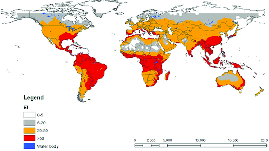
\includegraphics[width=5.5cm]{aux/climex_tuta.pdf}};
\node[font=\scriptsize,anchor=south east] at (climex.north east) {(Tonnang et al. 2015)};
%%
\node[subsection,anchor=north west,text width=8cm,shift={(1.3,0)}] (dataSrc)
at (ecoTitle.north east) {Leveraging diverse data types};
\node[body,anchor=north west,text width=6cm] (dataBody) at (dataSrc.south
west |- ecoBody.north east) {
   \begin{itemize}
      \item geographic distribution of crop production
      \item biology of the pest, host
      \item climate
      \item import, export
      \item domestic logistics
      \item market prices
      \item surveys
   \end{itemize}
};
%% sep line
\draw[blue2] ($(dataSrc.north west)+(-.1,.1)$) -- +(0,-5);
\draw[blue2] ($(dataSrc.north west)+(-.1,.1)$) -- +(4,0);
%%
\node[fig,anchor=south east,shift={(2.3,0)}] (metroInv) at (dataBody.south
east|-climex.south east) {\includegraphics[width=2.5cm]{aux/metro_invasive.png}};
\node[fig,shift={(0,0)},anchor=south east] (cfs) at (metroInv.south west) {\includegraphics[width=2.5cm]{aux/cfs.png}};
\node[fig,anchor=south east] (cropscape) at (cfs.north east) {\includegraphics[width=2.5cm]{aux/cropscape.png}};
\node[fig,anchor=south east] (ams) at (metroInv.north east) {\includegraphics[width=2.5cm]{aux/ams.png}};
\node[fig,anchor=south east] (ers) at (ams.north east) {\includegraphics[width=2.5cm]{aux/ers.png}};
\node[fig,anchor=south east] (fao) at (ers.north east) {\includegraphics[width=2.5cm]{aux/faostat.png}};
\node[fig,anchor=south east] (searates) at (cropscape.north east) {\includegraphics[width=2.5cm]{aux/searates.png}};
%%
\node[subsection,anchor=north west,shift={(.5,0)}] (comp)
at (dataSrc.north-|metroInv.east) {Computational problems of interest};
\node[body,anchor=north west,text width=6.8cm] (compBody) at (comp.south
west) {
   This approach has the potential to raise new questions which could be of
   interest to the data mining community. Also, several well-studied
   research topics can be revisited from the perspective of plant
   disease epidemiology. Some examples are as follows:
   \begin{itemize}[topsep=4pt]
      \item network inference
      \item community detection
      \item optimal quarantining
      \item optimal placement of traps
      \item link prediction
   \end{itemize}
};
\draw[blue2] (climex.south-|botRight.east) -- +(0,5);
\draw[blue2] (climex.south-|botRight.east) -- +(-4,0);
%%
\node[section,font=\huge,text width=18cm,anchor=north west,shift={(0,-.5)}]
(tuta) at (climex.south west) {The South American tomato leafminer
\emph{Tuta absoluta}};
\secLine{tuta}{20cm}
%%
\node[body,shift={(6.1,0)},text width=9cm] at (tuta.south west)
(tutaBody) {
\begin{itemize}
   \item A devastating tomato pest
   \item Found in packaging material, and survives harsh winters and
   summers in greenhouses
   \item 50-100\% crop loss
   \item Attacks other plants in the \emph{Solanaceae} family: potato,
   eggplant, pepper, tobacco.
   \item Health costs: In Spain, in the first year of introduction, pesticides were
   applied 15 times per season.
   \item Financial costs: When T. absoluta invades rest of the world, the
   tomato pest management cost will go up by \$500~M per year.
   \item Societal costs: In West Africa alone, more than 500,000 farmers
   make their living by growing tomatoes.
\end{itemize}
};
%%
\node[anchor=north west,fig,shift={(0,-.5)}] (adult) at (tuta.north
west|-tutaBody.north) {\includegraphics[width=3cm]{aux/tuta_adult.png}};
\node[anchor=north west,fig,shift={(2.6,-1.6)}] (larva) at (adult.north west)
{\includegraphics[width=3cm]{aux/tuta_larva.png}};
\node[anchor=north west,fig,shift={(0,-.6)}] (damage) at (adult.south west)
{\includegraphics[width=3cm]{aux/tomato_damage.png}};
\node[anchor=south west,fig,shift={(0,-.1)}] (field) at (larva.south
west|-botRight.south)
{\includegraphics[width=3cm]{aux/damaged_field_kenya.png}};
\node[fig,anchor=south east] (timeline) at (botRight.south east)
{\includegraphics[width=7.5cm]{aux/tuta_timeline_expanded.pdf}};
\node[font=\scriptsize,anchor=south east] at (timeline.north east) {The
   timeline of \tuta{} expansion (From EPPO, literature \& pers. comm.)};
%% team & contact
   \node[block,anchor=south west,minimum height=4.5cm,minimum width=10.6cm,rounded corners=0cm, thick,
draw=blue2] at (topLeft.west|-botRight.south) {};
\node[anchor=south west] (qr) at (topLeft.west|-botRight.south)
{\includegraphics[width=1.2cm]{aux/spread_qrcode.pdf}};
\node[right of=qr,shift={(3,-.2)},font=\large] (url)
{\parbox[t]{6cm}{abhijin@vbi.vt.edu\\https://www.bi.vt.edu/ndssl/projects/spread}};
%%
\node[body,anchor=south west] (ack) at (qr.north west){This work is partially supported
by a grant from the IPM Innovation Lab funded by United States Agency for
International Development Cooperative Agreement No.
AID-OAA-L-15-00001.};
\node[section,font=\Large,anchor=south west,shift={(0,1)}] (partners) at
(ack.north west) {Partners};
\node[anchor=west,shift={(0,-.5)}] (inra) at (partners.south west) {\includegraphics[width=3cm]{aux/inra.png}};
\node[right=of inra,shift={(-1,0)}] (cirad) {\includegraphics[width=3cm]{aux/cirad.png}};
\node[right=of cirad,shift={(-1,0)}] (iihr)
{\includegraphics[width=2cm]{aux/iihr.png}};
%%
%% linking text to modules
\draw[blue2] (approach-|modelTitle.west)+(-2,0) node[acceptSmall] {} -|
($(modelTitle.west)+(-.5,0)$) -- +(0.3,0) node[accept] {};
\draw[blue2] (case-|tuta.west)+(-2,0) node[acceptSmall] {} -|
($(tuta.west)+(-.5,0)$) -- +(0.3,0) node[accept] {};
%%
\draw[blue2] (modelFig.south east)+(-.4,2) node[acceptSmall] {} -|
($(netTitle.west)+(-.5,0)$) -- +(0.3,0) node[accept] {};
\draw[blue2] (modelFig.south west)+(1.8,.4) node[acceptSmall] {} |- 
($(ecoTitle.north east)+(0,.2)$) -- +(0,-0.5) node[accept] {};
\end{tikzpicture}
\end{document}
